%%%%%%%%%%%%%%%%%%%%%%%%%%%%%%%%%%%%%%%%%
%  My documentation report
%  Objective: Explain what I did and how, in order to help someone continue with the investigation
%
% Important note:
% Chapter heading images should have a 2:1 width:height ratio,
% e.g. 920px width and 460px height.
%
% The images can be found anywhere, usually on sky surveys websites or the
% Astronomy Picture of the day archive http://apod.nasa.gov/apod/archivepix.html
%
% The original template (the Legrand Orange Book Template) can be found here --> http://www.latextemplates.com/template/the-legrand-orange-book
%
% Original author of the Legrand Orange Book Template:
% Mathias Legrand (legrand.mathias@gmail.com) with modifications by:
% Vel (vel@latextemplates.com)
%
% Original License:
% CC BY-NC-SA 3.0 (http://creativecommons.org/licenses/by-nc-sa/3.0/)
%%%%%%%%%%%%%%%%%%%%%%%%%%%%%%%%%%%%%%%%%
 
%----------------------------------------------------------------------------------------
%	PACKAGES AND OTHER DOCUMENT CONFIGURATIONS
%----------------------------------------------------------------------------------------

\documentclass[11pt,fleqn]{book} % Default font size and left-justified equations

\usepackage[top=3cm,bottom=3cm,left=3.2cm,right=3.2cm,headsep=10pt,letterpaper]{geometry} % Page margins

\usepackage{xcolor} % Required for specifying colors by name
\definecolor{ocre}{RGB}{52,177,201} % Define the orange color used for highlighting throughout the book

% Font Settings
\usepackage{avant} % Use the Avantgarde font for headings
%\usepackage{times} % Use the Times font for headings
\usepackage{mathptmx} % Use the Adobe Times Roman as the default text font together with math symbols from the Sym­bol, Chancery and Com­puter Modern fonts

\usepackage{microtype} % Slightly tweak font spacing for aesthetics
\usepackage[utf8]{inputenc} % Required for including letters with accents
\usepackage[T1]{fontenc} % Use 8-bit encoding that has 256 glyphs

\usepackage{type1cm}
\usepackage{lettrine}

% Bibliography
\usepackage[style=alphabetic,sorting=nyt,sortcites=true,autopunct=true,babel=hyphen,hyperref=true,abbreviate=false,backref=true,backend=biber]{biblatex}
\addbibresource{bibliography.bib} % BibTeX bibliography file
\defbibheading{bibempty}{}

%%%%%%%%%%%%%%%%%%%%%%%%%%%%%%%%%%%%%%%%%
% This is based on the Legrand Orange Book
% Structural Definitions File
%
% The original template (the Legrand Orange Book Template) can be found here --> http://www.latextemplates.com/template/the-legrand-orange-book
%
% Original author of the Legrand Orange Book Template::
% Mathias Legrand (legrand.mathias@gmail.com) with modifications by:
% Vel (vel@latextemplates.com)
%
% Original License:
% CC BY-NC-SA 3.0 (http://creativecommons.org/licenses/by-nc-sa/3.0/)
%
%%%%%%%%%%%%%%%%%%%%%%%%%%%%%%%%%%%%%%%%%
%----------------------------------------------------------------------------------------
%	VARIOUS REQUIRED PACKAGES
%----------------------------------------------------------------------------------------

\usepackage{titlesec} % Allows customization of titles

\usepackage{graphicx} % Required for including pictures
\graphicspath{{Pictures/}} % Specifies the directory where pictures are stored

\usepackage{lipsum} % Inserts dummy text

\usepackage{tikz} % Required for drawing custom shapes

\usepackage[english]{babel} % English language/hyphenation

\usepackage{enumitem} % Customize lists
\setlist{nolistsep} % Reduce spacing between bullet points and numbered lists

\usepackage{booktabs} % Required for nicer horizontal rules in tables

\usepackage{eso-pic} % Required for specifying an image background in the title page

%----------------------------------------------------------------------------------------
%	MAIN TABLE OF CONTENTS
%----------------------------------------------------------------------------------------

\usepackage{titletoc} % Required for manipulating the table of contents

\contentsmargin{0cm} % Removes the default margin
% Chapter text styling
\titlecontents{chapter}[1.25cm] % Indentation
{\addvspace{15pt}\large\sffamily\bfseries} % Spacing and font options for chapters
{\color{ocre!60}\contentslabel[\Large\thecontentslabel]{1.25cm}\color{ocre}} % Chapter number
{}  
{\color{ocre!60}\normalsize\sffamily\bfseries\;\titlerule*[.5pc]{.}\;\thecontentspage} % Page number
% Section text styling
\titlecontents{section}[1.25cm] % Indentation
{\addvspace{5pt}\sffamily\bfseries} % Spacing and font options for sections
{\contentslabel[\thecontentslabel]{1.25cm}} % Section number
{}
{\sffamily\hfill\color{black}\thecontentspage} % Page number
[]
% Subsection text styling
\titlecontents{subsection}[1.25cm] % Indentation
{\addvspace{1pt}\sffamily\small} % Spacing and font options for subsections
{\contentslabel[\thecontentslabel]{1.25cm}} % Subsection number
{}
{\sffamily\;\titlerule*[.5pc]{.}\;\thecontentspage} % Page number
[] 

%----------------------------------------------------------------------------------------
%	MINI TABLE OF CONTENTS IN CHAPTER HEADS
%----------------------------------------------------------------------------------------

% Section text styling
\titlecontents{lsection}[0em] % Indendating
{\footnotesize\sffamily} % Font settings
{}
{}
{}

% Subsection text styling
\titlecontents{lsubsection}[.5em] % Indentation
{\normalfont\footnotesize\sffamily} % Font settings
{}
{}
{}
 
%----------------------------------------------------------------------------------------
%	PAGE HEADERS
%----------------------------------------------------------------------------------------

\usepackage{fancyhdr} % Required for header and footer configuration

\pagestyle{fancy}
\renewcommand{\chaptermark}[1]{\markboth{\sffamily\normalsize\bfseries\chaptername\ \thechapter.\ #1}{}} % Chapter text font settings
\renewcommand{\sectionmark}[1]{\markright{\sffamily\normalsize\thesection\hspace{5pt}#1}{}} % Section text font settings
\fancyhf{} \fancyhead[LE,RO]{\sffamily\normalsize\thepage} % Font setting for the page number in the header
\fancyhead[LO]{\rightmark} % Print the nearest section name on the left side of odd pages
\fancyhead[RE]{\leftmark} % Print the current chapter name on the right side of even pages
\renewcommand{\headrulewidth}{0.5pt} % Width of the rule under the header
\addtolength{\headheight}{2.5pt} % Increase the spacing around the header slightly
\renewcommand{\footrulewidth}{0pt} % Removes the rule in the footer
\fancypagestyle{plain}{\fancyhead{}\renewcommand{\headrulewidth}{0pt}} % Style for when a plain pagestyle is specified

% Removes the header from odd empty pages at the end of chapters
\makeatletter
\renewcommand{\cleardoublepage}{
\clearpage\ifodd\c@page\else
\hbox{}
\vspace*{\fill}
\thispagestyle{empty}
\newpage
\fi}

%----------------------------------------------------------------------------------------
%	THEOREM STYLES
%----------------------------------------------------------------------------------------

\usepackage{amsmath,amsfonts,amssymb,amsthm} % For math equations, theorems, symbols, etc

\newcommand{\intoo}[2]{\mathopen{]}#1\,;#2\mathclose{[}}
\newcommand{\ud}{\mathop{\mathrm{{}d}}\mathopen{}}
\newcommand{\intff}[2]{\mathopen{[}#1\,;#2\mathclose{]}}
\newtheorem{notation}{Notation}[chapter]

%%%%%%%%%%%%%%%%%%%%%%%%%%%%%%%%%%%%%%%%%%%%%%%%%%%%%%%%%%%%%%%%%%%%%%%%%%%
%%%%%%%%%%%%%%%%%%%% dedicated to boxed/framed environements %%%%%%%%%%%%%%
%%%%%%%%%%%%%%%%%%%%%%%%%%%%%%%%%%%%%%%%%%%%%%%%%%%%%%%%%%%%%%%%%%%%%%%%%%%
\newtheoremstyle{ocrenumbox}% % Theorem style name
{0pt}% Space above
{0pt}% Space below
{\normalfont}% % Body font
{}% Indent amount
{\small\bf\sffamily\color{ocre}}% % Theorem head font
{\;}% Punctuation after theorem head
{0.25em}% Space after theorem head
{\small\sffamily\color{ocre}\thmname{#1}\nobreakspace\thmnumber{\@ifnotempty{#1}{}\@upn{#2}}% Theorem text (e.g. Theorem 2.1)
\thmnote{\nobreakspace\the\thm@notefont\sffamily\bfseries\color{black}---\nobreakspace#3.}} % Optional theorem note
\renewcommand{\qedsymbol}{$\blacksquare$}% Optional qed square

\newtheoremstyle{blacknumex}% Theorem style name
{5pt}% Space above
{5pt}% Space below
{\normalfont}% Body font
{} % Indent amount
{\small\bf\sffamily}% Theorem head font
{\;}% Punctuation after theorem head
{0.25em}% Space after theorem head
{\small\sffamily{\tiny\ensuremath{\blacksquare}}\nobreakspace\thmname{#1}\nobreakspace\thmnumber{\@ifnotempty{#1}{}\@upn{#2}}% Theorem text (e.g. Theorem 2.1)
\thmnote{\nobreakspace\the\thm@notefont\sffamily\bfseries---\nobreakspace#3.}}% Optional theorem note

\newtheoremstyle{blacknumbox} % Theorem style name
{0pt}% Space above
{0pt}% Space below
{\normalfont}% Body font
{}% Indent amount
{\small\bf\sffamily}% Theorem head font
{\;}% Punctuation after theorem head
{0.25em}% Space after theorem head
{\small\sffamily\thmname{#1}\nobreakspace\thmnumber{\@ifnotempty{#1}{}\@upn{#2}}% Theorem text (e.g. Theorem 2.1)
\thmnote{\nobreakspace\the\thm@notefont\sffamily\bfseries---\nobreakspace#3.}}% Optional theorem note

%%%%%%%%%%%%%%%%%%%%%%%%%%%%%%%%%%%%%%%%%%%%%%%%%%%%%%%%%%%%%%%%%%%%%%%%%%%
%%%%%%%%%%%%% dedicated to non-boxed/non-framed environements %%%%%%%%%%%%%
%%%%%%%%%%%%%%%%%%%%%%%%%%%%%%%%%%%%%%%%%%%%%%%%%%%%%%%%%%%%%%%%%%%%%%%%%%%
\newtheoremstyle{ocrenum}% % Theorem style name
{5pt}% Space above
{5pt}% Space below
{\normalfont}% % Body font
{}% Indent amount
{\small\bf\sffamily\color{ocre}}% % Theorem head font
{\;}% Punctuation after theorem head
{0.25em}% Space after theorem head
{\small\sffamily\color{ocre}\thmname{#1}\nobreakspace\thmnumber{\@ifnotempty{#1}{}\@upn{#2}}% Theorem text (e.g. Theorem 2.1)
\thmnote{\nobreakspace\the\thm@notefont\sffamily\bfseries\color{black}---\nobreakspace#3.}} % Optional theorem note
\renewcommand{\qedsymbol}{$\blacksquare$}% Optional qed square
\makeatother

% Defines the theorem text style for each type of theorem to one of the three styles above
\newcounter{dummy} 
\numberwithin{dummy}{section}
\theoremstyle{ocrenumbox}
\newtheorem{theoremeT}[dummy]{Theorem}
\newtheorem{problem}{Problem}[chapter]
\newtheorem{exerciseT}{Exercise}[chapter]
\theoremstyle{blacknumex}
\newtheorem{exampleT}{Example}[chapter]
\theoremstyle{blacknumbox}
\newtheorem{vocabulary}{Vocabulary}[chapter]
\newtheorem{definitionT}{Definition}[section]
\newtheorem{corollaryT}[dummy]{Corollary}
\theoremstyle{ocrenum}
\newtheorem{proposition}[dummy]{Proposition}

%----------------------------------------------------------------------------------------
%	DEFINITION OF COLORED BOXES
%----------------------------------------------------------------------------------------

\RequirePackage[framemethod=default]{mdframed} % Required for creating the theorem, definition, exercise and corollary boxes

% Theorem box
\newmdenv[skipabove=7pt,
skipbelow=7pt,
backgroundcolor=black!5,
linecolor=ocre,
innerleftmargin=5pt,
innerrightmargin=5pt,
innertopmargin=5pt,
leftmargin=0cm,
rightmargin=0cm,
innerbottommargin=5pt]{tBox}

% Exercise box	  
\newmdenv[skipabove=7pt,
skipbelow=7pt,
rightline=false,
leftline=true,
topline=false,
bottomline=false,
backgroundcolor=ocre!10,
linecolor=ocre,
innerleftmargin=5pt,
innerrightmargin=5pt,
innertopmargin=5pt,
innerbottommargin=5pt,
leftmargin=0cm,
rightmargin=0cm,
linewidth=4pt]{eBox}	

% Definition box
\newmdenv[skipabove=7pt,
skipbelow=7pt,
rightline=false,
leftline=true,
topline=false,
bottomline=false,
linecolor=ocre,
innerleftmargin=5pt,
innerrightmargin=5pt,
innertopmargin=0pt,
leftmargin=0cm,
rightmargin=0cm,
linewidth=4pt,
innerbottommargin=0pt]{dBox}	

% Corollary box
\newmdenv[skipabove=7pt,
skipbelow=7pt,
rightline=false,
leftline=true,
topline=false,
bottomline=false,
linecolor=gray,
backgroundcolor=black!5,
innerleftmargin=5pt,
innerrightmargin=5pt,
innertopmargin=5pt,
leftmargin=0cm,
rightmargin=0cm,
linewidth=4pt,
innerbottommargin=5pt]{cBox}

% Creates an environment for each type of theorem and assigns it a theorem text style from the "Theorem Styles" section above and a colored box from above
\newenvironment{theorem}{\begin{tBox}\begin{theoremeT}}{\end{theoremeT}\end{tBox}}
\newenvironment{exercise}{\begin{eBox}\begin{exerciseT}}{\hfill{\color{ocre}\tiny\ensuremath{\blacksquare}}\end{exerciseT}\end{eBox}}				  
\newenvironment{definition}{\begin{dBox}\begin{definitionT}}{\end{definitionT}\end{dBox}}	
\newenvironment{example}{\begin{exampleT}}{\hfill{\tiny\ensuremath{\blacksquare}}\end{exampleT}}		
\newenvironment{corollary}{\begin{cBox}\begin{corollaryT}}{\end{corollaryT}\end{cBox}}	

%----------------------------------------------------------------------------------------
%	REMARK ENVIRONMENT
%----------------------------------------------------------------------------------------

\newenvironment{remark}{\par\vspace{10pt}\small % Vertical white space above the remark and smaller font size
\begin{list}{}{
\leftmargin=35pt % Indentation on the left
\rightmargin=25pt}\item\ignorespaces % Indentation on the right
\makebox[-2.5pt]{\begin{tikzpicture}[overlay]
\node[draw=ocre!60,line width=1pt,circle,fill=ocre!25,font=\sffamily\bfseries,inner sep=2pt,outer sep=0pt] at (-15pt,0pt){\textcolor{ocre}{R}};\end{tikzpicture}} % Orange R in a circle
\advance\baselineskip -1pt}{\end{list}\vskip5pt} % Tighter line spacing and white space after remark

%----------------------------------------------------------------------------------------
%	SECTION NUMBERING IN THE MARGIN
%----------------------------------------------------------------------------------------

\makeatletter
\renewcommand{\@seccntformat}[1]{\llap{\textcolor{ocre}{\csname the#1\endcsname}\hspace{1em}}}                    
\renewcommand{\section}{\@startsection{section}{1}{\z@}
{-4ex \@plus -1ex \@minus -.4ex}
{1ex \@plus.2ex }
{\normalfont\large\sffamily\bfseries}}
\renewcommand{\subsection}{\@startsection {subsection}{2}{\z@}
{-3ex \@plus -0.1ex \@minus -.4ex}
{0.5ex \@plus.2ex }
{\normalfont\sffamily\bfseries}}
\renewcommand{\subsubsection}{\@startsection {subsubsection}{3}{\z@}
{-2ex \@plus -0.1ex \@minus -.2ex}
{.2ex \@plus.2ex }
{\normalfont\small\sffamily\bfseries}}                        
\renewcommand\paragraph{\@startsection{paragraph}{4}{\z@}
{-2ex \@plus-.2ex \@minus .2ex}
{.1ex}
{\normalfont\small\sffamily\bfseries}}

%----------------------------------------------------------------------------------------
%	HYPERLINKS IN THE DOCUMENTS
%----------------------------------------------------------------------------------------

% For an unclear reason, the package should be loaded now and not later
\usepackage{hyperref}
\hypersetup{hidelinks,backref=true,pagebackref=true,hyperindex=true,colorlinks=false,breaklinks=true,urlcolor= ocre,bookmarks=true,bookmarksopen=false,pdftitle={Title},pdfauthor={Author}}

%----------------------------------------------------------------------------------------
%	CHAPTER HEADINGS
%----------------------------------------------------------------------------------------

% The set-up below should be (sadly) manually adapted to the overall margin page septup controlled by the geometry package loaded in the main.tex document. It is possible to implement below the dimensions used in the goemetry package (top,bottom,left,right)... TO BE DONE

\newcommand{\thechapterimage}{}
\newcommand{\chapterimage}[1]{\renewcommand{\thechapterimage}{#1}}

% Numbered chapters with mini tableofcontents
\def\thechapter{\arabic{chapter}}
\def\@makechapterhead#1{
\thispagestyle{empty}
{\centering \normalfont\sffamily
\ifnum \c@secnumdepth >\m@ne
\if@mainmatter
\startcontents
\begin{tikzpicture}[remember picture,overlay]
\node at (current page.north west)
{\begin{tikzpicture}[remember picture,overlay]
\node[anchor=north west,inner sep=0pt] at (0,0) {\includegraphics[width=\paperwidth]{\thechapterimage}};
%%%%%%%%%%%%%%%%%%%%%%%%%%%%%%%%%%%%%%%%%%%%%%%%%%%%%%%%%%%%%%%%%%%%%%%%%%%%%%%%%%%%%
% Commenting the 3 lines below removes the small contents box in the chapter heading
%\fill[color=ocre!10!white,opacity=.6] (1cm,0) rectangle (8cm,-7cm);
%\node[anchor=north west] at (1.1cm,.35cm) {\parbox[t][8cm][t]{6.5cm}{\huge\bfseries\flushleft \printcontents{l}{1}{\setcounter{tocdepth}{2}}}};
\draw[anchor=west] (5cm,-9cm) node [rounded corners=20pt,fill=ocre!10!white,text opacity=1,draw=ocre,draw opacity=1,line width=1.5pt,fill opacity=.6,inner sep=12pt]{\huge\sffamily\bfseries\textcolor{black}{\thechapter. #1\strut\makebox[22cm]{}}};
%%%%%%%%%%%%%%%%%%%%%%%%%%%%%%%%%%%%%%%%%%%%%%%%%%%%%%%%%%%%%%%%%%%%%%%%%%%%%%%%%%%%%
\end{tikzpicture}};
\end{tikzpicture}}
\par\vspace*{230\p@}
\fi
\fi}

% Unnumbered chapters without mini tableofcontents (could be added though) 
\def\@makeschapterhead#1{
\thispagestyle{empty}
{\centering \normalfont\sffamily
\ifnum \c@secnumdepth >\m@ne
\if@mainmatter
\begin{tikzpicture}[remember picture,overlay]
\node at (current page.north west)
{\begin{tikzpicture}[remember picture,overlay]
\node[anchor=north west,inner sep=0pt] at (0,0) {\includegraphics[width=\paperwidth]{\thechapterimage}};
\draw[anchor=west] (5cm,-9cm) node [rounded corners=20pt,fill=ocre!10!white,fill opacity=.6,inner sep=12pt,text opacity=1,draw=ocre,draw opacity=1,line width=1.5pt]{\huge\sffamily\bfseries\textcolor{black}{#1\strut\makebox[22cm]{}}};
\end{tikzpicture}};
\end{tikzpicture}}
\par\vspace*{230\p@}
\fi
\fi
}
\makeatother % Insert the commands.tex file which contains the majority of the structure behind the template

\pagenumbering{num_style}

\usepackage{fancyhdr}
\usepackage{lipsum}

% Turn on the style
\pagestyle{fancy}
% Clear the header and footer
\fancyhead{}
\fancyfoot{}
% Set the right side of the footer to be the page number
\fancyfoot[R]{\thepage}

\begin{document}
\title{Smart Real Estate Assessment}

%----------------------------------------------------------------------------------------
%	TITLE PAGE
%----------------------------------------------------------------------------------------

\begingroup
\thispagestyle{empty}
\AddToShipoutPicture*{\put(0,0){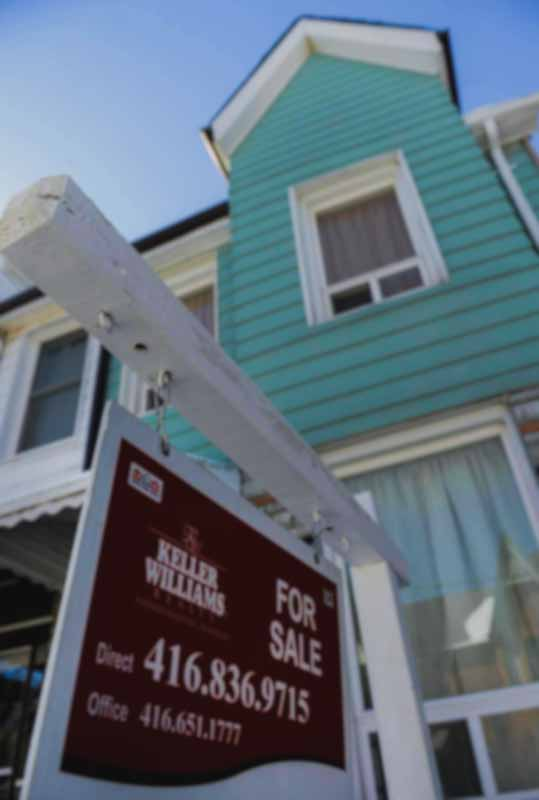
\includegraphics[scale=1.25]{front.jpg}}} % Image background
\centering
\vspace*{1cm}
\par\normalfont\fontsize{40}{35}\sffamily\selectfont\color{white}
{\LARGE A Preliminary Project Report on}\par 
\vspace*{4cm}
\textbf{SMART REAL ESTATE ASSESSMENT}\\ % Project title
\vspace*{4cm}
{\large Presented By}\par
\vspace*{1cm}
{\Huge Patne Nikhil}\par
{\Huge Shinde Abhishek}\par
{\Huge Gholap Satyawan}\par
{\Huge Dange Namrata}\par
{\Huge Beera Vivechana}\par
\endgroup

%----------------------------------------------------------------------------------------
%	COPYRIGHT PAGE
%----------------------------------------------------------------------------------------

\newpage
~\vfill
\thispagestyle{empty}
\vspace{-5cm}
\begin{center}
	  \begin{figure}[h]
			\centering
			
\includegraphics[width=5 cm]{Pictures/coem.png}
		\end{figure}
	  \fontsize{10}{10}\textbf{\LARGE DEPARTMENT OF COMPUTER ENGINEERING}\\
	  SVPM'S COLLEGE OF ENGINEERING\\
	  MALEGAON(Bk) \\
	   2018-19
	  \end{center}
	 \vspace{0cm}
\begin{center}
\text{\LARGE Sponsored by}
	  \begin{figure}[h]
			\centering
			
\includegraphics[width=5 cm]{Pictures/xento_logo_1200X630.jpg}
		\end{figure}
	  \end{center}
	  \begin{center}
	      \text{Xento Systems Private Limited, Pune}
	  \end{center}
\vspace{2cm}
%\noindent Copyright \copyright\ 2014 Andrea Hidalgo\\ % Copyright notice

\noindent \textsc{SVPM's College of Engineering Malegaon(Bk.) Baramati}\\
\noindent \textsc{github.com/AbhieShinde/Project}\\ % URL
\noindent This research was done under the guidance of Prof. Nimbalkar S.S. and Prof. Khumbhar H.R. with in the sponsorship of Xento Systems Pvt. Ltd., Pune, from August 2018.\\ % License information

%----------------------------------------------------------------------------------------
%	CERTIFICATE
%----------------------------------------------------------------------------------------
\newpage


\begin{figure}[ht]
\centering

\includegraphics[scale=0.4]{Pictures/coem.png}
\end{figure}


{\bfseries \fontsize{14}{12} \selectfont \centerline{SVPM's COLLEGE OF ENGINEERING}
\centerline{DEPARTMENT OF COMPUTER ENGINEERING}
\vspace*{1.2\baselineskip}} 


{\bfseries \fontsize{20}{20} \selectfont \centerline{\color{ocre} CERTIFICATE} 
\vspace*{1.4\baselineskip}} 

\centerline{This is to certify that the Project Entitled}
\vspace*{1\baselineskip} 


{\bfseries \fontsize{20}{12} \selectfont \centerline{\color{ocre}\LARGE Smart Real Estate Assessment}
\vspace*{1\baselineskip}}

\centerline{Submitted by}
\vspace*{0.72\baselineskip} 
\centerline{\LARGE Dange Namrata Milind \hspace{25 mm} Exam No:B150194\textbf{\color{ocre}206}}
\vspace{2mm}
\centerline{\LARGE Gholap Satywan Ashok \hspace{24 mm} Exam No:B150194\textbf{\color{ocre}214}}
\vspace{2mm}
\centerline{\LARGE Patne Nikhil Sunil \hspace{37 mm} Exam No:B150194\textbf{\color{ocre}234}}
\vspace{2mm}
\centerline{\LARGE Shinde Abhishek Sunil \hspace{26 mm} Exam No:B150194\textbf{\color{ocre}242}}
\vspace{2mm}
\centerline{\LARGE Beera Vivechana Ramesh \hspace{20 mm} Exam No:B150194\textbf{\color{ocre}259}}
\vspace*{1\baselineskip} 
is a bonafide work carried out by Students under the supervision of\\ \textbf{\LARGE\color{ocre} Prof. Nimbalkar S.S.} and it
is submitted towards the partial fulfillment of the requirement of Bachelor of Engineering (Computer Engineering) Project.\\[1cm]

\bgroup
\def\arraystretch{0.7}
\begin{tabular}{c c }
\vspace{2mm}
Prof.Nimbalkar S.S &  \hspace{40 mm} Prof.Kumbhar H.R \\								
\vspace{2mm}
Internal Guide   &  \hspace{40 mm} H.O.D \\[2cm]
\vspace{0.1cm}\_\_\_\_\_\_\_\_\_\_\_\_\_\_\_\_\_\_\_\_\_\_\_\_ & \hspace{40 mm} \_\_\_\_\_\_\_\_\_\_\_\_\_\_\_\_\_\_\_\_\_\_\_\_\\
External Examiner &\hspace{40 mm}Principal\\
\end{tabular}\\[1cm]
Place : SVPM's COE Malegaon(Bk.)\\
Date  : 


%----------------------------------------------------------------------------------------
%	Acknowledgments
%----------------------------------------------------------------------------------------
\newpage
\bfseries \fontsize{15}{19} \normalfont \centerline{\LARGE\color{ocre} Acknowledgments} 
			          \pagestyle{empty}
			         {\setlength{\baselineskip}{2\baselineskip}}
			         
\textit{It gives us great pleasure in presenting the preliminary project report 
on {\bfseries \fontsize{12}{12} \color{ocre} `Smart Real Estate Assessment'}.}
\vspace*{1.5\baselineskip}

 \textit{I would like to take this opportunity to thank my internal guide
 \textbf{Prof. Nimbalkar S.S}  and all teachers for giving me all the help and guidance I needed. I am
 really grateful to them for their kind support.I appreciate all valuable suggestions given  and queries raised by her which really helped us in exploring project in deep.} \vspace*{1.5\baselineskip}

 \textit{I am also grateful to \textbf{\color{ocre}Prof.Kumbhar H.R}, Head of Computer
 Engineering Department, SVPM COE for his indispensable
 support, suggestions.}
\vspace*{1.5\baselineskip}

\textit{In the end our special thanks to \textbf{\color{ocre}Mr.Nimbalkar S.S} for
providing various resources such as  laboratory with all needed software platforms,
continuous Internet connection, for Our Project.}
\vspace*{3\baselineskip} \\

\begin{flushright}
\begin{tabular}{p{8.2cm}c}
&\hspace{6 mm}Dange Namrata\\
&\hspace{8 mm}Gholap Satywan\\
&Patne Nikhil\\
&\hspace{9mm}Shinde Abhishek\\
&\hspace{9mm}Beera Vivechana\\[1cm]
&\hspace{7 mm}(B.E. Computer Engg.)

\end{tabular}
\end{flushright}

\maketitle
\addcontentsline{toc}{section}{Acknowledgment}


\newpage
\bfseries \fontsize{15}{19} \normalfont \centerline{\LARGE\color{ocre} Abstract} 
			          \pagestyle{empty}
			         {\setlength{\baselineskip}{2\baselineskip}
			         
\paragraph*{}\lettrine[lines=2]{\color{ocre!60} R}{eal} estate appraisal, which is the process of estimating the price for real estate properties, is crucial for both buys and sellers as the basis for negotiation and transaction. Traditionally, the repeat sales model has been widely adopted to estimate real estate price. However, it depends the design and calculation of a complex economic related index, which is challenging to estimate accurately. Today, real estate brokers provide easy access to detailed online information on real estate properties to their clients. We are interested in estimating the real estate price from these large amounts of easily accessed data. In particular, we analyze the prediction power of online house pictures, which is one of the key factors for online users to make a potential visiting decision. The development of robust computer vision algorithms makes the analysis of visual content possible. In this work, we employ a Recurrent Neural Network (RNN) to predict real estate price using the state-of-the-art visual features.\\
In a smart city, effective and accurate real estate assessments governed by a local government is crucial for determining the property taxes. Such assessments have never been trivial, and inappropriate assessments may result in disputes between property owners and the local government.\\
Generally for price prediction \textbf{\color{ocre} Regression} is used (Prediction of continuos valued-function). But here we are going to use \textbf{\color{ocre} Structured Deep Neural Network} in order to improve efficiency and accuracy. We introduce a deep learning approach to smartly and effectively assessing real estate values. We propose a systematic method to derive a layered knowledge graph and design a structured Deep Neural Network (DNN) based on it. Neurons in a structured DNN are structurally connected, which makes the network time and space efficient; and thus, it requires fewer data points for training. The structured DNN model has been designed to learn from the most recently captured data points; therefore, it allows the model to adapt to the latest market trends.

 \addcontentsline{toc}{section}{Abstract}
			         }


%----------------------------------------------------------------------------------------
%	TABLE OF CONTENTS
%----------------------------------------------------------------------------------------

\chapterimage{index.png} % Table of contents heading image

\pagestyle{empty} % No headers

\tableofcontents % Print the table of contents itself

%\cleardoublepage % Forces the first chapter to start on an odd page so it's on the right

\pagestyle{fancy} % Print headers again

%----------------------------------------------------------------------------------------
%	Lists
%----------------------------------------------------------------------------------------
\newpage
\chapterimage{figure.png}
			         \pagestyle{empty}
                     \pagenumbering{roman}
			         {\setlength{\baselineskip}{1.5\baselineskip}
			         \listoffigures
			         \addcontentsline{toc}{section}{List of Figures}
			         }
			         
\newpage
\chapterimage{table_edited.jpg}
			          \pagestyle{empty}
			         {\setlength{\baselineskip}{1.5\baselineskip}
			         \listoftables
			         \addcontentsline{toc}{section}{List of Tables}
			         }
%----------------------------------------------------------------------------------------
%	CHAPTER 1
%----------------------------------------------------------------------------------------

\chapterimage{syn.jpg} % Chapter heading image

\chapter{Synopsis}

\section{Project Title}\index{Project Title}
\textbf{\LARGE\color{ocre}\textit{Smart Real Estate Assessment}}

\section{ Project Option}\index{ Project Option}
\emph{Internal project}

\section{Internal Guide}\index{Guide}
\emph{\LARGE Prof.Nimbalkar S.S}

\section{Sponsorship and External Guide}\index{Sponsorship}
\textbf{\LARGE\color{ocre}\textit{Xento Systems Private Limited, Pune}}
    \item Mr. Amol Deshpande
    \item Mr. Mayur Narole
    \item Mr. Anand Chandole
    
    
    
\section{Problem Statement}
\label{sec:problem}
To predict the price of the real estate properties which is depends upon various factors like Infrastructure,Neighbourhood environment,House age, Location etc. using Structured Deep Neural Network.

\section{Goals and Objectives}
\subsection{Goal}
	\item To construct an assessment system using Deep Neural Network in a more efficient & effective way with, improved accuracy for house-price prediction.

\subsection{Objectives}
	\begin{itemize}
	\item Prediction of prices of real estate property more accurately(Using DNN).
	\item Elimination of Role of Middle Person(\emph{Agent}).
	\item Assessments are not only for urban areas but also for Rular areas.
\end{itemize}



%\begin{remark}
%For more information about the cosmological principle, review Chapter 1: Why Learn Astronomy?, page 10, from \textbf{21st Century Astronomy}, \textit{Hester | Smith | Blumenthal | Kay | Voss}, Third Edition, 2010.
%\end{remark}

%This statement requires citation \cite{book_key}; this one is more specific \cite[122]{article_key}.


%----------------------------------------------------------------------------------------
%	CHAPTER 2
%----------------------------------------------------------------------------------------
\chapterimage{techkey.jpg}

\chapter{Technical Keywords}

\section{Area of Project}
\textbf{\color{ocre}Deep Neural Network}
\begin{figure}[h]
    \centering
    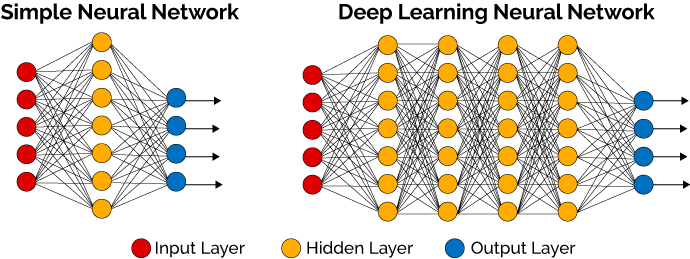
\includegraphics[width=0.77\textwidth]{Pictures/dnn.png}
    \caption{Difference between Simple Neural Network and Deep Neural Network, https://becominghuman.ai/deep-learning-made-easy-with-deep-cognition-403fbe445351}
    \label{fig:awesome_image}
\end{figure}

%	\begin{verbatim}
% 	$ vi .profile
%  \end{verbatim}


\section{Technical Keywords}\
\begin{enumerate}
    \item \textbf{\LARGE\color{ocre}Deep Learning}:  Deep learning is an aspect of artificial intelligence (AI) that is concerned with emulating the learning approach that human beings use to gain certain types of knowledge. At its simplest, deep learning can be thought of as a way to automate predictive analytics.Deep learning is the branch of machine learning which having ability to learn multiple level representation from structured data using supervised or unsupervised learning.
    \vspace{2mm}
    \item \textbf{\LARGE\color{ocre}Personalization}: Personalization goes more with the user's decisions, this means, the instructions explicitly given. An example could be the background image of twitter could be taken as personalization of your twitter profile.
    \vspace{2mm}
	\item \textbf{\LARGE\color{ocre}Online Interest}: Get users interest through social media like twitter,facebook.For that data need to mine.
	\vspace{2mm}
	\item \textbf{\LARGE\color{ocre}Social Media}: To  mine users point of interest need to get data from usesrs social account.

 \end{enumerate}

%----------------------------------------------------------------------------------------
%	CHAPTER 3
%----------------------------------------------------------------------------------------

\chapterimage{3introduction.jpg}
\chapter{Introduction}

\section{Project Idea}

    
%\begin{table}[h]
%  \centering
%  \begin{tabular}{ c c c c c c }
 %   \hline\hline
  %  Filter / Config. & Waveband / Central $\lambda$/ Line & Obs. Date & Comment \\
  %  \hline
 %   F225W & UV filter / 235.9 nm & 26 Aug 2009 &  UV wide\\
    
%    F336W & UV filter / 335.5 nm & 26 Aug 2009 & Str$\ddot{o}$mgren $u$\\
    
   % F373N & Narrow-Band Filter / 373.0 nm & 19 Aug 2009 & Includes \textsc{[OII]}\\
    
  %  F438W & Wide-Band Filter / 432.5 nm & 26 Aug 2009 & $B$, Johnson-Cousins set\\
    
  %  F487N & Narrow-Band Filter / 487.1 nm & 25 Aug 2009 & Includes H$\beta$\\
    
 %   F502N & Narrow-Band Filter / 501.0 nm & 26 Aug 2009 & Includes \textsc{[O III]}\\
%    
    %F657N & Narrow-Band Filter / 656.7 nm & 25 Aug 2009 & Includes %H$\alpha$+\textsc{[NII]}\\
 %   
%    F673N & Narrow-Band Filter / 676.6 nm & 20 Aug 2009 & Includes \textsc{[SII]}\\
%    
%    F814W & Wide-Band Filter / 802.4 nm & 26 Aug 2009 & $I$, Johnson-Cousins set\\
   % \hline
  %\end{tabular}
  %\caption{Summary of Observations}
 % \label{tab:uno}
%\end{table}

%-------------------------------------------------------------
\section{Motivation of the Project}

\section{Literature Survey}

%----------------------------------------------------------------------------------------
%	CHAPTER 4
%----------------------------------------------------------------------------------------
\chapterimage{}
\chapter{}

\section{}

%----------------------------------------------------------------------------------------
%	CHAPTER 5
%----------------------------------------------------------------------------------------
\chapterimage{}
\chapter{}

\section{}

%----------------------------------------------------------------------------------------
%	CHAPTER 6
%----------------------------------------------------------------------------------------
\chapterimage{}
\chapter{}

\section{}

%----------------------------------------------------------------------------------------
%	CHAPTER 7
%----------------------------------------------------------------------------------------
\chapterimage{}
\chapter{}

\section{}

%----------------------------------------------------------------------------------------
%	CHAPTER 8
%----------------------------------------------------------------------------------------

\chapterimage{}
\chapter{}

\section{}

%--------------------------------------------------------------------------
\end{document}